\documentclass{article}
\usepackage{fancyhdr}
\usepackage{ctex}
\usepackage{listings}
\usepackage{graphicx}
\usepackage[a4paper, body={18cm,22cm}]{geometry}
\usepackage{amsmath,amssymb,amstext,wasysym,enumerate,graphicx}
\usepackage{float,abstract,booktabs,indentfirst,amsmath}
\usepackage{array}
\usepackage{booktabs}
\usepackage{multirow}
\usepackage{url}
\usepackage{diagbox}
\renewcommand\arraystretch{1.4}
\usepackage{indentfirst}
\setlength{\parindent}{2em}
\usepackage{enumitem}
\setmonofont{Consolas}
\usepackage{listings}
\usepackage{xcolor}
\usepackage{makecell}
\usepackage{tikz}
\usetikzlibrary{positioning, arrows.meta}
\setCJKmonofont{黑体}
\lstset{  
	% 基本设置  
	xleftmargin = 3em, xrightmargin = 3em, aboveskip = 1em,  
	backgroundcolor = \color{white},  
	basicstyle = \small\ttfamily,  
	rulesepcolor = \color{gray},  
	breaklines = true,  
	numbers = left,  
	numberstyle = \small,  
	numbersep = -14pt,  
	frame = shadowbox,  
	showspaces = false,  
	columns = fixed,  
	sensitive = true,  
	% VSCode 风格配色  
	keywordstyle = \color{blue!70!black}\bfseries,  
	emphstyle = \color{red!70!black}\bfseries, % 对于强调的词  
	emphstyle=[2]\color{purple!70!black}\bfseries, % 对于第二组强调的词  
	commentstyle = \color{green!60!black}, % 注释颜色  
	stringstyle = \color{orange!90!black}, % 字符串颜色更亮一些  
	morekeywords={ASSERT, int64\_t, uint32\_t},  
	moreemph={ASSERT, NULL},  
	moreemph=[2]{int64\_t, uint32\_t, tid\_t, uint8\_t, int16\_t, uint16\_t, int32\_t, size\_t, bool},  
	morecomment=[l][\color{green!60!black}]{+}, % 以+开头的注释  
}

%--------------------页眉--------------------%
\pagestyle{fancy}
\fancyhead[L]{}
\fancyhead[R]{}
\fancyhead[C]{华东师范大学软件工程学院}
\fancyfoot[C]{-\thepage-}
\renewcommand{\headrulewidth}{1.5pt}
%--------------------标题--------------------%
\begin{document}
\begin{center}
	{\Large{\textbf{\heiti 第九讲作业——基于组件的软件可信性度量模型}}}
	\begin{table}[H]
		\centering
		\begin{tabular}{p{2cm}p{4cm}<{\centering}p{1cm}p{2cm}p{6cm}<{\centering}}
			课程名称:    & 软件质量分析 & \quad & 指导教师:    & 陈仪香
			\\ \cline{2-2} \cline{5-5}
			姓\qquad 名: & 王海生    & \quad & 学\qquad 号: & 10235101559
			\\ \cline{2-2} \cline{5-5}
			年\qquad 级: & 2023级    & \quad & 主\qquad 题: & 游戏服务器系统的可信度量
			\\ \cline{2-2} \cline{5-5}
		\end{tabular}
	\end{table}
	
	% 添加新行并居中
	%\vspace{1em} % 可选:添加垂直间距
\end{center}
\rule{\textwidth}{1pt}

\tableofcontents

%--------------------正文--------------------%
\section{题目要求}
\begin{enumerate}
	\item 编程实现基于组件的软件可信性度量模型。
	\item 游戏服务器系统包含13个组件,分别是网关组件(\(cp1\))、游戏大厅组件(\(cp2\))、公共 组件(\(cp3\))、配置组件(\(cp4\))、核心服务器组件(\(cp5\))、总捕鱼游戏组件(\(cp6\))、 用户捕鱼游戏组件(\(cp7\))、注册组件(\(cp8\))、游戏 \(AI\) 组件(\(cp9\))、后台管理组件 (\(cp10\))、工具组件(\(cp11\))、消息组件(\(cp12\))、\(Maven\) 插件组件(\(cp13\))。其中\(cp1 - cp5\)为关键组件, \(cp6 - cp12\)为非关键组件。 他们之间的正互反判断矩阵以及各组件的可信值见讲授\(ppt\)最后三页。 
	\item 计算在关键组件组与非关键组件组的权重分别取为\((\alpha, \beta)=(0.7, 0.3), (0.6, 0.4), (0.55, 0.45)\)的情况下,游戏服务器系统的可信度量值以及可信等级。
\end{enumerate}

\textbf{关键组件正互反判断矩阵及权重:}

\begin{center}
	\begin{tabular}{|c|c|c|c|c|c|c|}
		\hline
		组件名 & CP1 & CP2 & CP3 & CP4 & CP5 & 属性权重 \\
		\hline
		CP1 & 1 & 2 & 1/2 & 2 & 1/4 & \\
		\hline
		CP2 & 1/2 & 1 & 2 & 3 & 1/2 & \\
		\hline
		CP3 & 2 & 1/2 & 1 & 1 & 1/2 & \\
		\hline
		CP4 & 1/2 & 1/3 & 1 & 1 & 1/2 & \\
		\hline
		CP5 & 4 & 2 & 2 & 2 & 1 & \\
		\hline
	\end{tabular}
\end{center}

\textbf{非关键组件正互反判断矩阵及权重:}

\begin{center}
	\begin{tabular}{|c|c|c|c|c|c|c|c|c|c|}
		\hline
		组件名 & CP6 & CP7 & CP8 & CP9 & CP10 & CP11 & CP12 & CP13 & 属性权重 \\
		\hline
		CP6 & 1 & 3 & 2 & 1/2 & 2 & 1 & 3 & 3 & \\
		\hline
		CP7 & 1/3 & 1 & 2 & 1 & 2 & 2 & 2 & 2 & \\
		\hline
		CP8 & 1/2 & 1/2 & 1 & 1/2 & 1 & 1/2 & 3 & 3 & \\
		\hline
		CP9 & 2 & 1 & 2 & 1 & 3 & 1/2 & 3 & 3 & \\
		\hline
		CP10 & 1/2 & 1/2 & 1 & 1/3 & 1 & 1 & 2 & 2 & \\
		\hline
		CP11 & 1 & 1/2 & 2 & 2 & 1 & 1 & 2 & 2 & \\
		\hline
		CP12 & 1/3 & 1/2 & 1 & 1/3 & 1/2 & 1/2 & 1 & 2 & \\
		\hline
		CP13 & 1/3 & 1/2 & 2 & 1/3 & 1/2 & 1/2 & 1/2 & 1 & \\
		\hline
	\end{tabular}
\end{center}

\textbf{组件可信值:}

\begin{center}
	\begin{tabular}{|c|c|c|c|c|c|c|c|}
		\hline
		组件名 & CP1 & CP2 & CP3 & CP4 & CP5 & CP6 & CP7 \\
		\hline
		可信值 & 8.430 & 8.530 & 6.042 & 9.094 & 8.289 & 6.192 & 8.020 \\
		\hline
		组件名 & CP8 & CP9 & CP10 & CP11 & CP12 & CP13 & \\
		\hline
		可信值 & 7.984 & 8.713 & 9.211 & 7.777 & 7.897 & 8.075 & \\
		\hline
	\end{tabular}
\end{center}

\normalsize

\section{相关知识点}

\subsection{总体思路}

\begin{enumerate}
	\item 在基于组件的软件中,软件系统性能是其组件性能的反映。为了计算软件的可信性,先要计算出组件的可信性。
	\item 在本节课的PPT中,首先建立组件可信量化评估指标体系,将可信性分解成若干个可信属性,再将可信属性向下分解为可信证据,依据可信证据的不同组合构建度量元;
	\item 其次构建基于属性的组件可信度量模型;
	\item 然后构建基于组件的软件可信性度量模型。
\end{enumerate}

\subsection{基于组件的软件可信性度量模型}

\begin {enumerate}
\item 软件系统中有若干组件,组件可以分为两大类,即关键组件和非关键组件。
\item 关键组件是指一个软件必须具备的组件,该组件的可信性对系统整体可信性影响较大。
\item 非关键组件是指软件自身除了关键组件外可能还需要的其他组件。
\item 关键组件和非关键组件都能影响软件可信性。但关键组件更影响软件可信度量。
\item 设软件系统 $ S $ 有 $ n $ 个关键组件 $ FC_1, \cdots, FC_n $ 和 $ m $ 个非关键组件 $ NFC_1, \cdots, NFC_m $,关键组件的权重分别为 $ \alpha_1, \cdots, \alpha_n $,非关键组件的权重为 $ \beta_1, \cdots, \beta_m $。
\item 设关键组件和非关键组件的权重分别为 $ \alpha $ 和 $ \beta $,要求 $ \alpha > 1/2 > \beta > 0 $。
\item 组件间没有替换性。
\end{enumerate}

\textbf{基于组件的软件可信性度量模型的计算如下:}

\[ T_s = \alpha (FC_1^{\alpha_1} \times \cdots \times FC_n^{\alpha_n}) + \beta (NFC_1^{\beta_1} \times \cdots \times NFC_m^{\beta_m}) \]

\textbf{可信等级可以用下面表格中的方法确定:}

\begin{center}
	\begin{tabular}{|c|c|c|}
		\hline
		软件可信度量值要求 & 可信属性要求 & 可信等级 \\
		\hline
		$9.5 \leq T$ & 
		\begin{tabular}{l}
			1. 低于9.5分的关键组件个数 \\
			不超过 $n - [n \times 2/3]$ \\
			2. 没有低于8.5分的组件
		\end{tabular} & V \\
		\hline
		$8.5 \leq T < 9.5$ 或者 $T > 9.5$且不能评为V级别 & 
		\begin{tabular}{l}
			1. 低于8.5分的关键组件个数 \\
			不超过 $n - [n \times 2/3]$ \\
			2. 没有低于7.0分的组件
		\end{tabular} & IV \\
		\hline
		$7.0 \leq T < 8.5$ 或者 $T > 8.5$且不能评为IV级别及以上者 & 
		\begin{tabular}{l}
			1. 低于7.0分的关键组件个数 \\
			不超过 $n - [n \times 2/3]$ \\
			2. 没有低于4.5分的可信属性
		\end{tabular} & III \\
		\hline
		$4.5 \leq T < 7.0$ 或者 $T > 7.0$且不能评为III级别及以上者 & 
		\begin{tabular}{l}
			1. 低于4.5分的关键组件个数 \\
			不超过 $n - [n \times 2/3]$
		\end{tabular} & II \\
		\hline
		$T < 4.5$ 或者 $T > 4.5$且不能评为II级别及以上者 & 无要求 & I \\
		\hline
	\end{tabular}
\end{center}

\subsection{拓展:层次分析法}

\subsubsection{基本原理}

层次分析法(Analytic Hierarchy Process, AHP)是由美国运筹学家托马斯·萨蒂(Thomas L. Saaty)在20世纪70年代提出的一种用于多准则决策的数学工具。它通过将复杂的问题结构化,分解为一个层次化的模型,并利用两两比较的方式评估各元素之间的相对重要性,从而计算出各个属性或因素的权重。

在AHP中,正互反判断矩阵是表示成对比较结果的矩阵,具有以下特性:
\begin{itemize}
	\item 它是一个方阵,假设我们有$n$个属性,则矩阵大小为$n \times n$。
	\item 矩阵中的元素$a_{ij}$表示第$i$个属性相对于第$j$个属性的重要性比率,通常使用Saaty的1-9标度来量化。
	\item 对角线上的元素总是1,因为每个属性相对于自身的比较结果应该是相等的。
	\item 它满足互反性,即如果$a_{ij} = k$,则$a_{ji} = 1/k$。
\end{itemize}

\subsubsection{属性权重的计算}

为了从正互反判断矩阵计算属性的权重,可以遵循以下步骤:

\textbf{步骤 1:构建判断矩阵。}
根据专家意见或相关数据,建立所有属性之间的成对比较矩阵。

\textbf{步骤 2:计算几何平均值。}
对于每一行,计算其所有元素的几何平均值。对于第$i$行,权重$w_i$可以通过下面的公式计算:
$ w_i = \left( a_{i1} \times a_{i2} \times \dots \times a_{in} \right)^{\frac{1}{n}} $

\textbf{步骤 3:归一化处理。}
由于几何平均值可能不会自然地形成一个总和为1的权重向量,因此需要进行归一化处理。归一化后的权重$W_i$可以通过下面的公式计算:
$ W_i = \frac{w_i}{\sum_{k=1}^{n} w_k} $

\textbf{步骤 4:一致性检验。}
计算一致性比率(Consistency Ratio, CR),以检验判断矩阵的一致性。如果CR小于0.1,一般认为判断矩阵具有满意的一致性;否则,可能需要重新评估和调整判断矩阵。一致性指标(Consistency Index, CI)和随机一致性指标(Random Consistency Index, RI)用于计算CR:
$ CR = \frac{CI}{RI} $
其中CI由最大特征根$\lambda_{max}$得出,而RI依赖于矩阵的维度并且是预定义的。

\textbf{步骤 5:确定权重。}
如果一致性检验通过,那么归一化后的向量即为最终的权重向量,代表了每个属性的相对重要性。

\subsubsection{属性间相对重要性的量化}

Saaty的1-9标度提供了一种量化属性间相对重要性的方法,具体如下:
\begin{itemize}
	\item 1 表示两个属性同等重要;
	\item 3 表示一个属性稍微重要于另一个;
	\item 5 表示一个属性明显重要于另一个;
	\item 7 表示一个属性强烈重要于另一个;
	\item 9 表示一个属性极端重要于另一个;
	\item 2, 4, 6, 8 是上述相邻判断的中间值;
	\item 倒数用于表示相反的重要性关系。
\end{itemize}

\normalsize

\section{题目解析}

\subsection{计算关键组件和非关键组件的属性权重}

\textbf{代码:}

\begin{lstlisting}[language=Python]
	import numpy as np
	
	# 计算属性权重的函数,传入正互反判断矩阵
	def calculate_attribute_weights(matrix):
		n = matrix.shape[0]
		
		# 计算几何平均值
		geometric_means = np.power(np.prod(matrix, axis=1), 1 / n)
		
		# 归一化处理
		weights = geometric_means / np.sum(geometric_means)
		return weights
	
	# 1) 计算关键组件和非关键组件的属性权重
	key_weights = calculate_attribute_weights(key_components_matrix)
	non_key_weights = calculate_attribute_weights(non_key_components_matrix)
	
	print("关键组件属性权重:", key_weights)
	print("非关键组件属性权重:", non_key_weights)
\end{lstlisting}

\textbf{计算结果:}

\begin{lstlisting}
	关键组件属性权重: [0.16020622 0.19957385 0.16020622 0.11195645 0.36805725]
	非关键组件属性权重: [0.18373096 0.1500157  0.10384807 0.18373096 0.09727315 0.14471694 0.07130095 0.06538326]
\end{lstlisting}

\

\textbf{将属性权重填入表格中:}

\

\textbf{关键组件正互反判断矩阵及权重:}

\begin{center}
	\begin{tabular}{|c|c|c|c|c|c|c|}
		\hline
		组件名 & CP1 & CP2 & CP3 & CP4 & CP5 & 属性权重 \\
		\hline
		CP1 & 1 & 2 & 1/2 & 2 & 1/4 & 0.16020622 \\
		\hline
		CP2 & 1/2 & 1 & 2 & 3 & 1/2 & 0.19957385 \\
		\hline
		CP3 & 2 & 1/2 & 1 & 1 & 1/2 & 0.16020622 \\
		\hline
		CP4 & 1/2 & 1/3 & 1 & 1 & 1/2 & 0.11195645 \\
		\hline
		CP5 & 4 & 2 & 2 & 2 & 1 & 0.36805725 \\
		\hline
	\end{tabular}
\end{center}

\textbf{非关键组件正互反判断矩阵及权重:}

\begin{center}
	\begin{tabular}{|c|c|c|c|c|c|c|c|c|c|}
		\hline
		组件名 & CP6 & CP7 & CP8 & CP9 & CP10 & CP11 & CP12 & CP13 & 属性权重 \\
		\hline
		CP6 & 1 & 3 & 2 & 1/2 & 2 & 1 & 3 & 3 & 0.18373096 \\
		\hline
		CP7 & 1/3 & 1 & 2 & 1 & 2 & 2 & 2 & 2 & 0.1500157 \\
		\hline
		CP8 & 1/2 & 1/2 & 1 & 1/2 & 1 & 1/2 & 3 & 3 & 0.10384807 \\
		\hline
		CP9 & 2 & 1 & 2 & 1 & 3 & 1/2 & 3 & 3 & 0.18373096 \\
		\hline
		CP10 & 1/2 & 1/2 & 1 & 1/3 & 1 & 1 & 2 & 2 & 0.09727315 \\
		\hline
		CP11 & 1 & 1/2 & 2 & 2 & 1 & 1 & 2 & 2 & 0.14471694 \\
		\hline
		CP12 & 1/3 & 1/2 & 1 & 1/3 & 1/2 & 1/2 & 1 & 2 & 0.07130095 \\
		\hline
		CP13 & 1/3 & 1/2 & 2 & 1/3 & 1/2 & 1/2 & 1/2 & 1 & 0.06538326 \\
		\hline
	\end{tabular}
\end{center}

\subsection{计算游戏服务器系统的可信度量值T\_s}

\textbf{代码:}

\begin{lstlisting}[language=Python]
	# 2) 计算游戏服务器系统的可信度量值T_s
	key_component_product = np.prod(np.power(component_trust_values[:5], key_weights))
	non_key_component_product = np.prod(np.power(component_trust_values[5:], non_key_weights))
	
	T_s = alpha * key_component_product + beta * non_key_component_product
	
	print(f"当(α, β)=({alpha}, {beta})时,可信度量值T_s:", T_s)
\end{lstlisting}

\textbf{计算结果:}

\begin{lstlisting}
	当(α, β)=(0.7, 0.3)时,可信度量值T_s: 7.968354549775479
	当(α, β)=(0.6, 0.4)时,可信度量值T_s: 7.948107650109263
	当(α, β)=(0.6, 0.4)时,可信度量值T_s: 7.948107650109263
\end{lstlisting}

\subsection{确定可信等级}

\textbf{代码:}

\begin{lstlisting}[language=Python]
	# 根据可信度量值确定可信等级的函数
	def determine_trust_level(T_s):
		if 9.5 <= T_s:
			return "V"
		elif 8.5 <= T_s < 9.5:
			return "IV"
		elif 7.0 <= T_s < 8.5:
			return "III"
		elif 4.5 <= T_s < 7.0:
			return "II"
		else:
			return "I"
	
	level = determine_trust_level(T_s)
	print(f"可信等级: {level}")
\end{lstlisting}

\textbf{计算结果:}

\begin{lstlisting}
	当(α, β)=(0.7, 0.3)时,可信度量值T_s: 7.968354549775479
	可信等级: III
	当(α, β)=(0.6, 0.4)时,可信度量值T_s: 7.948107650109263
	可信等级: III
	当(α, β)=(0.55, 0.45)时,可信度量值T_s: 7.937984200276155
	可信等级: III
\end{lstlisting}

\normalsize

\section{结果总结}

代码运行结果如下图所示:

\begin{figure}[H]
	\centering
	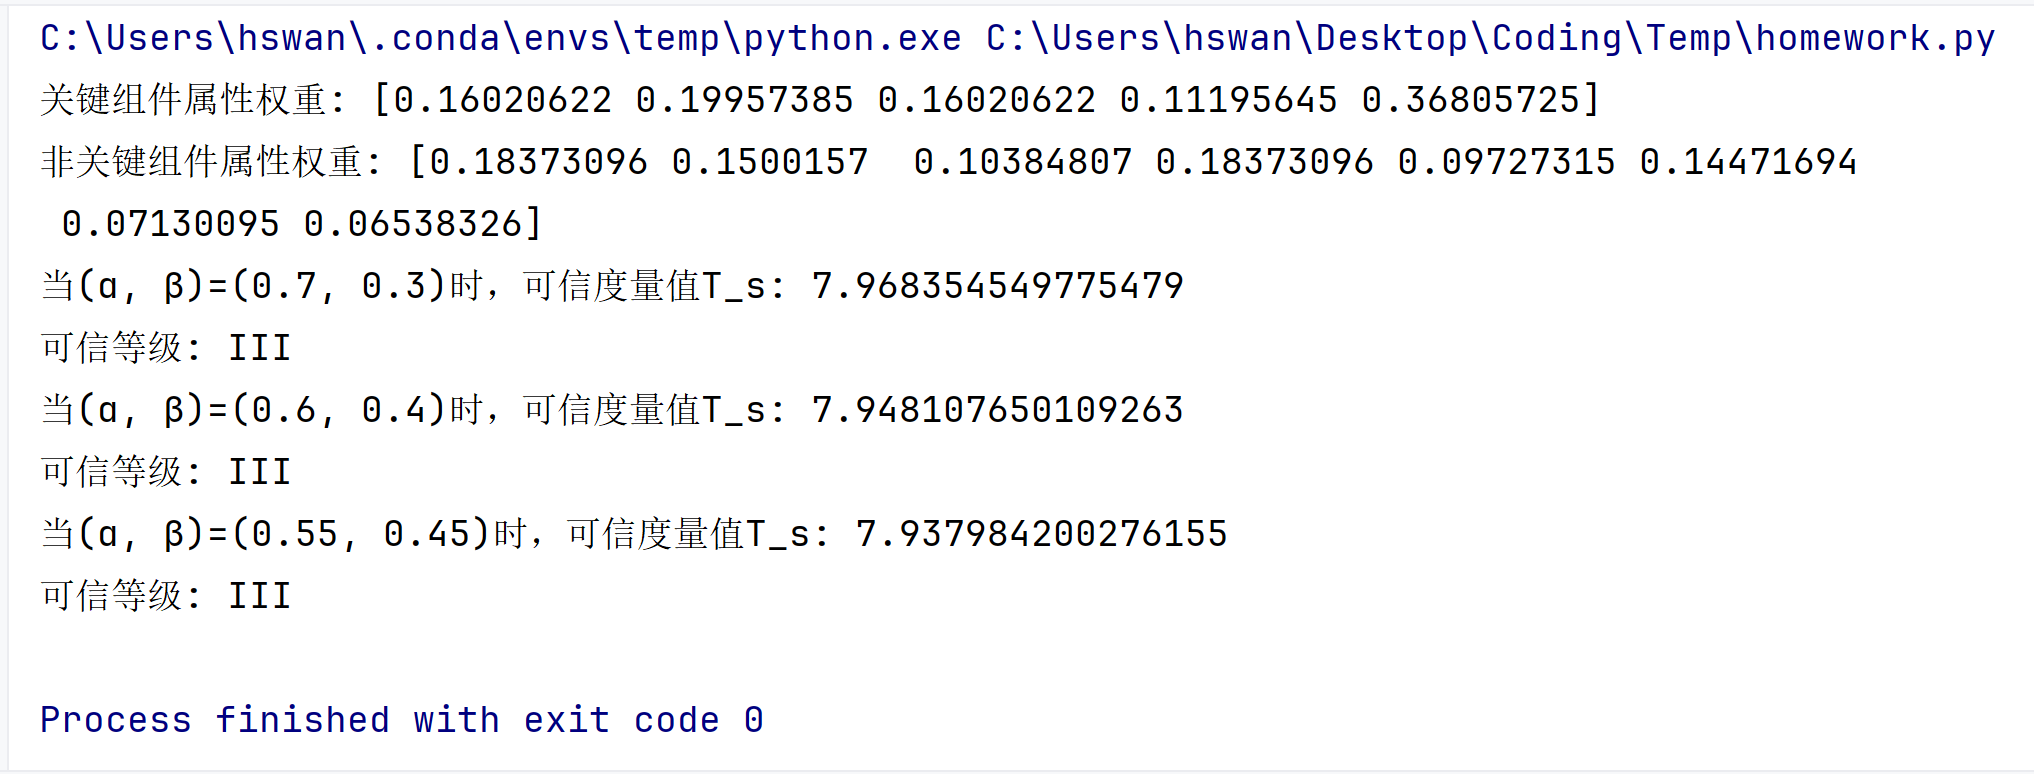
\includegraphics[width=0.9\textwidth]{img/1.png}
	\caption{运行结果}
\end{figure}

\normalsize

\section{完整代码}

\begin{lstlisting}[language=Python]
	import numpy as np
	
	
	# 计算属性权重的函数,传入正互反判断矩阵
	def calculate_attribute_weights(matrix):
		n = matrix.shape[0]
	
		# 计算几何平均值
		geometric_means = np.power(np.prod(matrix, axis=1), 1 / n)
		
		# 归一化处理
		weights = geometric_means / np.sum(geometric_means)
		return weights
	
	
	# 根据可信度量值确定可信等级的函数
	def determine_trust_level(T_s):
		if 9.5 <= T_s:
			return "V"
		elif 8.5 <= T_s < 9.5:
			return "IV"
		elif 7.0 <= T_s < 8.5:
			return "III"
		elif 4.5 <= T_s < 7.0:
			return "II"
		else:
			return "I"
	
	
	# 关键组件正互反判断矩阵
	key_components_matrix = np.array([
		[1, 2, 1 / 2, 2, 1 / 4],
		[1 / 2, 1, 2, 3, 1 / 2],
		[2, 1 / 2, 1, 1, 1 / 2],
		[1 / 2, 1 / 3, 1, 1, 1 / 2],
		[4, 2, 2, 2, 1]
	])
	
	# 非关键组件正互反判断矩阵
	non_key_components_matrix = np.array([
		[1, 3, 2, 1 / 2, 2, 1, 3, 3],
		[1 / 3, 1, 2, 1, 2, 2, 2, 2],
		[1 / 2, 1 / 2, 1, 1 / 2, 1, 1 / 2, 3, 3],
		[2, 1, 2, 1, 3, 1 / 2, 3, 3],
		[1 / 2, 1 / 2, 1, 1 / 3, 1, 1, 2, 2],
		[1, 1 / 2, 2, 2, 1, 1, 2, 2],
		[1 / 3, 1 / 2, 1, 1 / 3, 1 / 2, 1 / 2, 1, 2],
		[1 / 3, 1 / 2, 2, 1 / 3, 1 / 2, 1 / 2, 1 / 2, 1]
	])
	
	# 组件可信值
	component_trust_values = np.array([8.430, 8.530, 6.042, 9.094, 8.289, 6.192, 8.020,
	7.984, 8.713, 9.211, 7.777, 7.897, 8.075])
	
	# 1) 计算关键组件和非关键组件的属性权重
	key_weights = calculate_attribute_weights(key_components_matrix)
	non_key_weights = calculate_attribute_weights(non_key_components_matrix)
	
	print("关键组件属性权重:", key_weights)
	print("非关键组件属性权重:", non_key_weights)
	
	# 关键组件和非关键组件组的权重取值情况
	alpha_beta_list = [(0.7, 0.3), (0.6, 0.4), (0.55, 0.45)]
	for alpha, beta in alpha_beta_list:
	
	# 2) 计算游戏服务器系统的可信度量值T_s
	key_component_product = np.prod(np.power(component_trust_values[:5], key_weights))
	non_key_component_product = np.prod(np.power(component_trust_values[5:], non_key_weights))
	
	T_s = alpha * key_component_product + beta * non_key_component_product
	
	print(f"当(α, β)=({alpha}, {beta})时,可信度量值T_s:", T_s)
	
	# 3) 确定可信等级
	level = determine_trust_level(T_s)
	print(f"可信等级: {level}")
\end{lstlisting}

\normalsize

\end{document}